\documentclass[12pt]{article}
\usepackage[margin=1in]{geometry}
\usepackage{amsmath, amssymb, amsthm, graphicx, hyperref}
\usepackage{amsmath}
\usepackage{enumerate}
\usepackage{fancyhdr}
\usepackage{multirow, multicol}
\usepackage{tikz}
\usepackage{wrapfig}
\pagestyle{fancy}
\usepackage{titlesec}
\usepackage{lastpage}
\usepackage{multirow}
\usepackage{indentfirst}
\fancyhead[LO]{JACK Z}
\fancyhead[RO]{Page \thepage\ of \pageref{LastPage}}
\usepackage{comment}
\newtheorem{definition}{Definition}
\usepackage{amsmath}
\usepackage{booktabs}
\usepackage{xcolor}
\usepackage{tcolorbox}  % For creating styled boxes
\tcbuselibrary{most}
\usepackage{tcolorbox} % for creating colored or framed text boxes
\tcbuselibrary{breakable} % allows tcolorboxes to break across pages

\definecolor{examplebg}{RGB}{255, 228, 225} % Light red background
\tcbuselibrary{theorems} 
\usepackage{graphicx}
\usepackage{booktabs} % For better table formatting
\usepackage{caption} % Essential for \captionof
\usepackage{tcolorbox} % For creating colored boxes
\tcbuselibrary{most} % Load most libraries for tcolorbox

\newtcbtheorem[number within=subsection]{Note}{Note}{
    colback=Black!5,
    colframe=white!35!black,
    fonttitle=\bfseries,
    colbacktitle=blue!85!black,
    coltitle=white,
    enhanced,
    attach boxed title to top left={yshift=-2mm, xshift=2mm},
    boxed title style={sharp corners},
    sharp corners
}{Not}

\newtcbtheorem[number within=subsection]{Definition}{Definition}{
    colback=blue!5,
    colframe=blue!35!black,
    fonttitle=\bfseries,
    colbacktitle=blue!85!black,
    coltitle=white,
    enhanced,
    attach boxed title to top left={yshift=-2mm, xshift=2mm},
    boxed title style={sharp corners},
    sharp corners
}{def}

\newtcbtheorem[number within=subsection]{mytheorem}{Theorem}{
    colback=orange!5,      % Background color of the box
    colframe=orange,     % Border color of the box
    coltitle=white,     % Color of theorem title
    colbacktitle=orange!85!black,, % Background color for the title
    fonttitle=\bfseries,
    title after break={Theorem \csname the\tcbcounter\endcsname\ -- Continued}, % for continued theorems
    enhanced,
    attach boxed title to top left={yshift=-2mm, xshift=2mm},
    boxed title style={sharp corners, colframe=black},
    sharp corners,
    separator sign none % no sign between title and theorem text
}{thm}


\usepackage{lipsum} % 生成示例文本
\usepackage{fancyhdr}

\pagestyle{fancy}
\fancyfoot[C]{%
  \begin{tcolorbox}[colback=blue!10, colframe=blue!35, boxrule=0.5pt, 
  sharp corners=south, boxsep=2pt, width=0.25\textwidth, 
  arc=3mm, enhanced, shadow=drop shadow]
    \centering
    {\textbf{\textcopyright\ \textit{Novel Prep}}}
  \end{tcolorbox}
}

% Define custom colors
\definecolor{deepblue}{rgb}{0.0, 0.18, 0.39}
\definecolor{deepred}{rgb}{0.6, 0, 0}

% Define theorem style
\newtheoremstyle{beautifulthm}
  {10pt} % Space above
  {10pt} % Space below
  {\itshape} % Body font
  {} % Indent amount
  {\bfseries\color{deepblue}} % Theorem head font
  {.} % Punctuation after theorem head
  {.5em} % Space after theorem head
  {} % Theorem head spec

\theoremstyle{beautifulthm}
\newtheorem{theorem}{Theorem}[section]

\begin{document}

\title{AP Calculus AB\&BC}
\author{Hongjun Zeng}
\maketitle
\lipsum[1-10] 

\tableofcontents
\begin{document}
\section{Limits and Continuity}
\section{Differentiation: Definition and Fundamental Properties}
\section{Differentiation: Composite, Implicit, and Inverse Function}
\section{Application of Differentiation}
\section{Analytical Applications of Differentiation}
\newpage
\subsection{Rolle’s Theorem and the Mean Value Theorem}
\subsubsection{Rolle’s Theorem}
In the previous section, extreme Value Theorem states that a continuous function on a closed interval [a,b] must have both a minimum and a maximum on the interval. Both of these values, however, can occur at the endpoints. Rolle’s Theorem, gives conditions that guarantee the existence of an extreme value in the interior of a closed interval.
\begin{mytheorem}{Rolle's Theorem}{Squeeze Theorem}

Let \( f \) be continuous on the closed interval \([a, b]\) and differentiable on the open interval \((a, b)\). If \( f(a) = f(b) \), then there is at least one number \( c \) in \((a, b)\) such that \( f'(c) = 0 \).
\end{mytheorem}

\textbf{Note:} From Rolle's \textbf{Theorem}, you can see that if a function \( f \) is continuous on \([a, b]\) and differentiable on \((a, b)\), and if \( f(a) = f(b) \), then there must be at least one \( x \)-value between \( a \) and \( b \) at which the graph of \( f \) has a horizontal tangent (see Figure 5(a)). When the differentiability requirement is dropped from Rolle's \textbf{Theorem}, \( f \) will still have a critical number in \((a, b)\), but it may not yield a horizontal tangent. Such a case is shown in Figure 5(b).
\begin{minipage}{\linewidth}
    \centering
    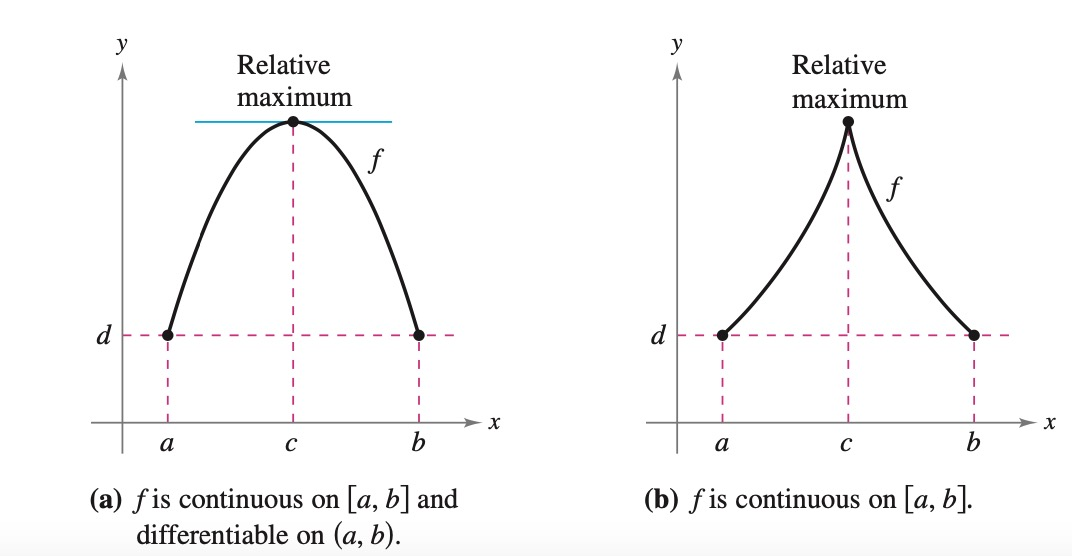
\includegraphics[width=0.800\linewidth]{Example_6.jpg} % Adjust the image width as necessary
    \captionof{figure}{}
    \label{fig:graph}
\end{minipage}

\begin{tcolorbox}[colback=examplebg, colframe=red!75!black, title=\textbf{EXAMPLE 1: Illustrating Rolle's Theorem}, fonttitle=\bfseries, sharp corners]
\textbf{
Find the two $x$-intercepts of
\[ f(x) = x^2 - 3x + 2 \]
and show that $f'(x) = 0$ at some point between the two $x$-intercepts.}
\tcblower
\textbf{Solution:} Note that $f$ is differentiable on the entire real number line. Setting $f(x)$ equal to 0 produces
\[ x^2 - 3x + 2 = 0 \]
\[ (x - 1)(x - 2) = 0 \]
\[ x = 1, 2. \]

So, $f(1) = f(2) = 0$, and from Rolle's Theorem, you know that there \textit{exists} at least one $c$ in the interval $(1, 2)$ such that $f'(c) = 0$. To \textit{find} such a $c$, differentiate $f$ to obtain
\[ f'(x) = 2x - 3 \]
and then determine that $f'(x) = 0$ when $x = \frac{3}{2}$. Note that this $x$-value lies in the open interval $(1, 2)$
\end{tcolorbox}
Rolle’s Theorem states that when f satisfies the conditions of the theorem, there must be at least one point between a and b at which the derivative is 0. There may, of course, be more than one such point, as shown in the next example.
\newpage
\subsubsection{Mean Value Theorem}
\text{Rolle’s Theorem can be used to prove another theorem—the Mean Value Theorem}
\begin{mytheorem}{Mean Value Theorem}{Squeeze Theorem}
If \( f \) is continuous on the closed interval \([a, b]\) and differentiable on the open interval \((a, b)\), then there exists a number \( c \) in \((a, b)\) such that

\[
f'(c) = \frac{f(b) - f(a)}{b - a}
\]
\begin{minipage}{\linewidth}
    \centering
    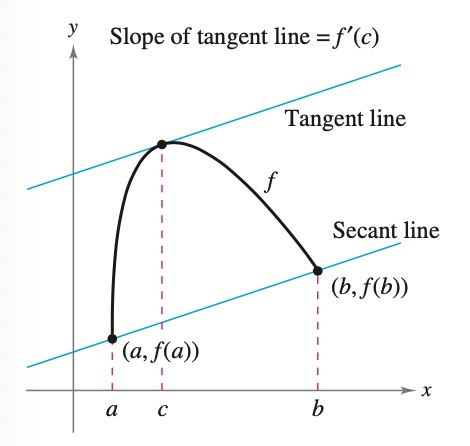
\includegraphics[width=0.325\linewidth]{Example_7.jpg} % Adjust the image width as necessary
    \captionof{figure}{}
    \label{fig:graph}
\end{minipage}
\end{mytheorem}
\begin{tcolorbox}[colback=examplebg, colframe=red!75!black, title=\textbf{EXAMPLE 2: Finding a Tangent Line}, fonttitle=\bfseries, sharp corners]
\textbf{
For \( f(x) = 5 - \frac{4}{x} \), find all values of \( c \) in the open interval \( (1, 4) \) such that
\[
f'(c) = \frac{f(4) - f(1)}{4 - 1}
\]

}
\tcblower
\textbf{Solution} The slope of the secant line through \( (1, f(1)) \) and \( (4, f(4)) \) is

\[
\frac{f(4) - f(1)}{4 - 1} = \frac{4 - 1}{4 - 1} = 1.
\]

\textit{Note} that the function satisfies the conditions of the \textbf{Mean Value Theorem}. That is, \( f \) is continuous on the interval \([1, 4]\) and differentiable on the interval \((1, 4)\). So, there exists at least one number \( c \) in \( (1, 4) \) such that \( f'(c) = 1 \). Solving the equation \( f'(x) = 1 \) yields

\[
\frac{4}{x^2} = 1
\]

which implies that

\[
x = \pm 2.
\]

So, in the interval \( (1, 4) \), you can conclude that \( c = 2 \)
\end{tcolorbox}

\subsection{Extrema on an Interval}
\subsubsection{Extrema of a Function}
\begin{Definition}{Definition of Extrema}{}
Let \( f \) be defined on an interval \( I \) containing \( c \):
\begin{enumerate}
    \item \( f(c) \) is the \textbf{minimum of \( f \) on \( I \)} when \( f(c) \leq f(x) \) for all \( x \) in \( I \).
    \item \( f(c) \) is the \textbf{maximum of \( f \) on \( I \)} when \( f(c) \geq f(x) \) for all \( x \) in \( I \).
\end{enumerate}

The minimum and maximum of a function on an interval are the \textbf{extreme values}, or \textbf{extrema} ), of the function on the interval. The minimum and maximum of a function on an interval are also called the \textbf{absolute minimum} and \textbf{absolute maximum}, or the \textbf{global minimum} and \textbf{global maximum}, on the interval. Extrema can occur at interior points or endpoints of an interval. Extrema that occur at the endpoints are called \textbf{endpoint extrema}.
\end{Definition}
\begin{minipage}{\linewidth}
    \centering
    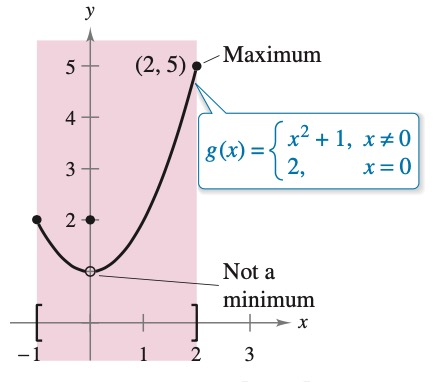
\includegraphics[width=0.45\linewidth]{Example_21.jpg} % Adjust the image width as necessary
    \captionof{figure}{}
    \label{fig:graph}
\end{minipage}
\begin{mytheorem}{The Extreme Value Theorem}{}
If \( f \) is continuous on a closed interval \([a, b]\), then \( f \) has both a minimum and a maximum on the interval.
\end{mytheorem}
\newpage


\subsubsection{Relative Extrema and Critical Numbers}
\begin{Definition}{Definition of Extrema}{}
Let \( f \) be defined on an interval \( I \) containing \( c \):
\begin{enumerate}
    \item If there is an open interval containing \( c \) on which \( f(c) \) is a maximum, then \( f(c) \) is called a \textbf{relative or local maximum} of \( f \), or you can say that \( f \) has a \textbf{relative or local maximum} at \( (c, f(c)) \).
    \item If there is an open interval containing \( c \) on which \( f(c) \) is a minimum, then \( f(c) \) is called a \textbf{relative or local minimum} of \( f \), or you can say that \( f \) has a \textbf{relative or local minimum} at \( (c, f(c)) \).
\end{enumerate}


\begin{minipage}{\linewidth}
    \centering
    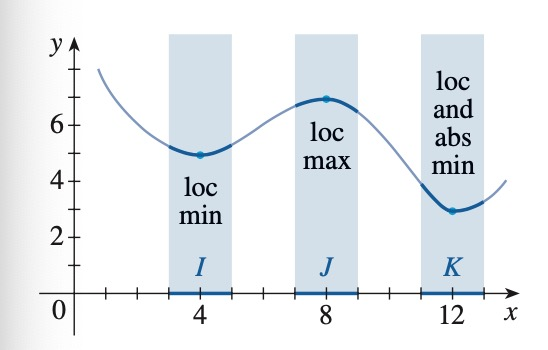
\includegraphics[width=0.35\linewidth]{Example_22.jpg} % Adjust the image width as necessary
    \captionof{figure}{}
    \label{fig:graph}
\end{minipage}
\end{Definition}

\begin{tcolorbox}[colback=examplebg, colframe=red!75!black, title=\textbf{EXAMPLE 1: Find the Local Min or Max}, fonttitle=\bfseries, sharp corners]
The graph of the function
\[
f(x) = 3x^4 - 16x^3 + 18x^2 \quad \text{for} \quad -1 \leq x \leq 4
\]
is shown

\begin{minipage}{\linewidth}
    \centering
    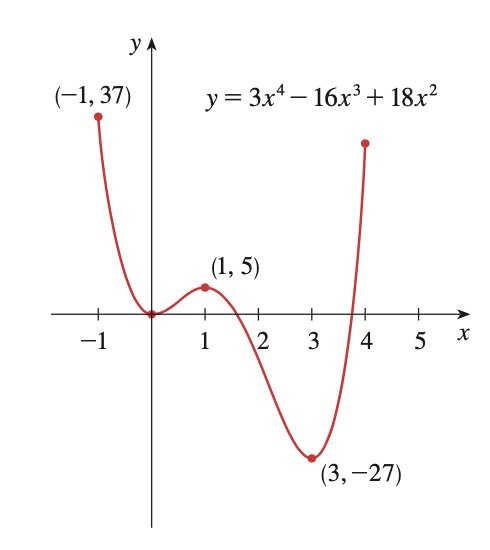
\includegraphics[width=0.30\linewidth]{Example_23.jpg} % Adjust the image width as necessary
    \captionof{figure}{}
    \label{fig:graph}
\end{minipage}
\tcblower
\textbf{Solution:} 
You can see that \( f(1) = 5 \) is a local maximum, whereas the absolute maximum is \( f(-1) = 37 \). Also, \( f(0) = 0 \) is a local minimum, and \( f(3) = -27 \) is both a local and an absolute minimum.
\end{tcolorbox}
\newpage
\begin{Definition}{Critical Number}{}
    Let \( f \) be defined at \( c \). If \( f'(c) = 0 \) or if \( f \) is not differentiable at \( c \), then \( c \) is a \textbf{critical number} of \( f \).
\end{Definition}

\begin{minipage}{\linewidth}
    \centering
    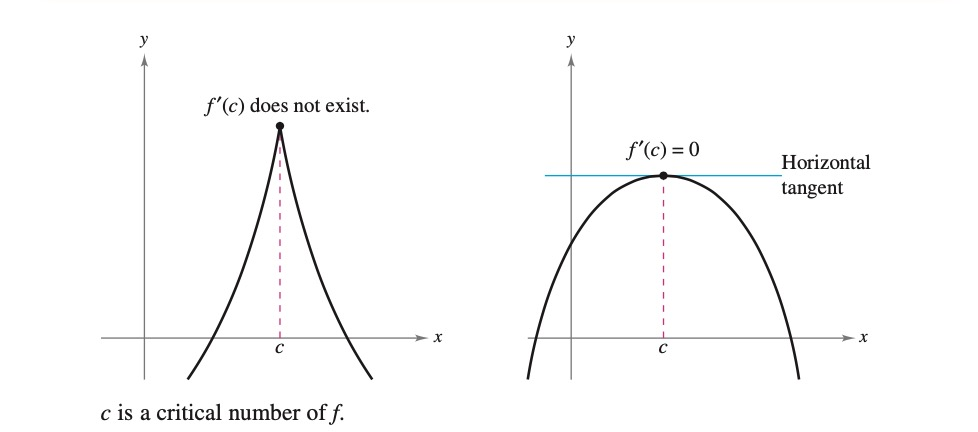
\includegraphics[width=0.80\linewidth]{Example_24.jpg} % Adjust the image width as necessary
    \captionof{figure}{}
    \label{fig:graph}
\end{minipage}

\begin{mytheorem}{Relative Extrema Occur Only at Critical Numbers}
If \( f \) has a relative minimum or relative maximum at \( x = c \), then \( c \) is a \textbf{critical number} of \( f \).
    
\end{mytheorem}
















\newpage
\subsubsection{Finding Extrema on a Closed Interval}

\begin{Note}{Guidelines for Finding Extrema on a Closed Interval}{}
To find the extrema of a continuous function \( f \) on a closed interval \([a, b]\), use these steps:
\begin{enumerate}
    \item Find the critical numbers of \( f \) in \((a, b)\).
    \item Evaluate \( f \) at each critical number in \((a, b)\).
    \item Evaluate \( f \) at each endpoint of \([a, b]\).
    \item The least of these values is the minimum. The greatest is the maximum.
\end{enumerate}
    
\end{Note}


\begin{tcolorbox}[colback=examplebg, colframe=red!75!black, title=\textbf{EXAMPLE 2: Find the Extrema}, fonttitle=\bfseries, sharp corners]
Find the extrema of
\[
f(x) = 3x^4 - 4x^3
\]
on the interval \([-1, 2]\).

\tcblower
\textbf{Solution:} 
Begin by differentiating the function:
\[
f(x) = 3x^4 - 4x^3 \quad \text{Write original function.}
\]
\[
f'(x) = 12x^3 - 12x^2 \quad \text{Differentiate.}
\]

To find the critical numbers of \( f \) in the interval \((-1, 2)\), you must find all \( x \)-values for which \( f'(x) = 0 \) and all \( x \)-values for which \( f'(x) \) does not exist:
\[
12x^3 - 12x^2 = 0 \quad \text{Set } f'(x) = 0.
\]
\[
12x^2(x - 1) = 0 \quad \text{Factor.}
\]
\[
x = 0, \, 1 \quad \text{Critical numbers.}
\]

Because \( f' \) is defined for all \( x \), you can conclude that these are the only critical numbers of \( f \). By evaluating \( f \) at these two critical numbers and at the endpoints of \([-1, 2]\), you can determine that the maximum is \( f(2) = 16 \) and the minimum is \( f(1) = -1 \), as shown in the table below. The graph of \( f \) is shown in Figure 3.5.

\textbf{Table of Values}
\[
\begin{array}{|c|c|c|c|}
\hline
\textbf{Left Endpoint} & \textbf{Critical Number} & \textbf{Critical Number} & \textbf{Right Endpoint} \\
\hline
f(-1) = 7 & f(0) = 0 & f(1) = -1 \, \text{(Minimum)} & f(2) = 16 \, \text{(Maximum)} \\
\hline
\end{array}
\]
\end{tcolorbox}

\subsection{Increasing and Decreasing Functions}
\begin{Definition}{Increasing and Decreasing Functions}
 A function \( f \) is \textbf{increasing} on an interval when, for any two numbers \( x_1 \) and \( x_2 \) in the interval, \( x_1 < x_2 \) implies \( f(x_1) < f(x_2) \).

A function \( f \) is \textbf{decreasing} on an interval when, for any two numbers \( x_1 \) and \( x_2 \) in the interval, \( x_1 < x_2 \) implies \( f(x_1) > f(x_2) \).   
\end{Definition}



\begin{minipage}{\linewidth}
    \centering
    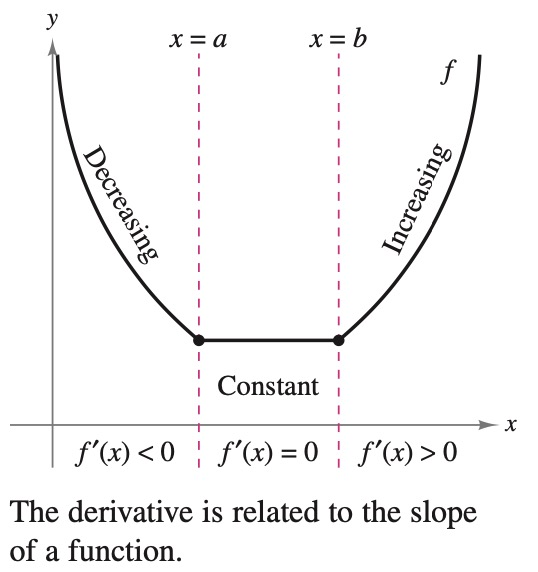
\includegraphics[width=0.50\linewidth]{Example_25.jpg} % Adjust the image width as necessary
    \captionof{figure}{}
    \label{fig:graph}
\end{minipage}


\begin{mytheorem}{Test for Increasing and Decreasing Functions}
Let \( f \) be a function that is continuous on the closed interval \( [a, b] \) and differentiable on the open interval \( (a, b) \).

\begin{enumerate}
    \item If \( f'(x) > 0 \) for all \( x \) in \( (a, b) \), then \( f \) is increasing on \( [a, b] \).
    \item If \( f'(x) < 0 \) for all \( x \) in \( (a, b) \), then \( f \) is decreasing on \( [a, b] \).
    \item If \( f'(x) = 0 \) for all \( x \) in \( (a, b) \), then \( f \) is constant on \( [a, b] \).
\end{enumerate}
\end{mytheorem}


\begin{tcolorbox}[colback=examplebg, colframe=red!75!black, title=\textbf{EXAMPLE 1: Intervals on Which \( f \) Is Increasing or Decreasing}, fonttitle=\bfseries, sharp corners]
Find the open intervals on which \( f(x) = x^3 - \frac{3}{2}x^2 \) is increasing or decreasing.
\tcblower
\textbf{Solution:} 
\quad Note that \( f \) is differentiable on the entire real number line and the derivative of \( f \) is
\[
f(x) = x^3 - \frac{3}{2}x^2 \quad \text{\textit{Write original function.}}
\]
\[
f'(x) = 3x^2 - 3x. \quad \text{\textit{Differentiate.}}
\]

To determine the critical numbers of \( f \), set \( f'(x) \) equal to zero:
\[
3x^2 - 3x = 0 \quad \text{\textit{Set \( f'(x) \) equal to 0.}}
\]
\[
3(x)(x - 1) = 0 \quad \text{\textit{Factor.}}
\]
\[
x = 0, 1 \quad \text{\textit{Critical numbers.}}
\]

Because there are no points for which \( f' \) does not exist, you can conclude that \( x = 0 \) and \( x = 1 \) are the only critical numbers. The table summarizes the testing of the three intervals determined by these two critical numbers.

\[
\begin{array}{|c|c|c|c|c|}
\hline
\textbf{Interval} & -\infty < x < 0 & 0 < x < 1 & 1 < x < \infty \\
\hline
\textbf{Test Value} & x = -1 & x = \frac{1}{2} & x = 2 \\
\hline
\textbf{Sign of \( f'(x) \)} & f'(-1) = 6 > 0 & f'\left( \frac{1}{2} \right) = -\frac{3}{4} < 0 & f'(2) = 6 > 0 \\
\hline
\textbf{Conclusion} & \text{Increasing} & \text{Decreasing} & \text{Increasing} \\
\hline
\end{array}
\]
\end{tcolorbox}

\begin{Note}{GUIDELINES FOR FINDING INTERVALS}{}
Let \( f \) be continuous on the interval \( (a, b) \). To find the open intervals on which \( f \) is increasing or decreasing, use the following steps.

\begin{enumerate}
    \item Locate the critical numbers of \( f \) in \( (a, b) \), and use these numbers to determine test intervals.
    \item Determine the sign of \( f'(x) \) at one test value in each of the intervals.
    \item Use Theorem to determine whether \( f \) is increasing or decreasing on each interval.
\end{enumerate}
    
\end{Note}

\newpage
\subsection{The First Derivative Test}
\begin{mytheorem}{The First Derivative Test}{}
    
Let \( c \) be a critical number of a function \( f \) that is continuous on an open interval \( I \) containing \( c \). If \( f \) is differentiable on the interval, except possibly at \( c \), then \( f(c) \) can be classified as follows.

\begin{enumerate}
    \item If \( f'(x) \) changes from negative to positive at \( c \), then \( f \) has a \textit{relative minimum} at \( (c, f(c)) \).
    \item If \( f'(x) \) changes from positive to negative at \( c \), then \( f \) has a \textit{relative maximum} at \( (c, f(c)) \).
    \item If \( f'(x) \) is positive on both sides of \( c \) or negative on both sides of \( c \), then \( f(c) \) is neither a relative minimum nor a relative maximum.
\end{enumerate}
\begin{minipage}{\linewidth}
    \centering
    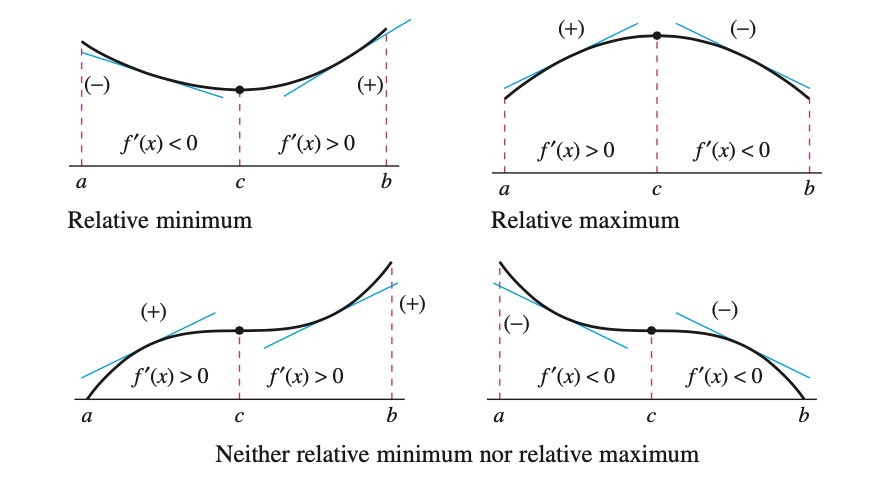
\includegraphics[width=0.80\linewidth]{Example_26.jpg} % Adjust the image width as necessary
    \captionof{figure}{}
    \label{fig:graph}
\end{minipage}
\end{mytheorem}


\begin{tcolorbox}[colback=examplebg, colframe=red!75!black, title=\textbf{EXAMPLE 1: Applying the First Derivative Test}, fonttitle=\bfseries, sharp corners]
Find the relative extrema of \( f(x) = \frac{1}{2}x - \sin x \) in the interval \( (0, 2\pi) \).
\tcblower
\textbf{Solution:} 
 \quad Note that \( f \) is continuous on the interval \( (0, 2\pi) \). The derivative of \( f \) is \( f'(x) = \frac{1}{2} - \cos x \). To determine the critical numbers of \( f \) in this interval, set \( f'(x) \) equal to 0:
\[
\frac{1}{2} - \cos x = 0 \quad \text{\textit{Set \( f'(x) \) equal to 0.}}
\]
\[
\cos x = \frac{1}{2}
\]
\[
x = \frac{\pi}{3}, \frac{5\pi}{3} \quad \text{\textit{Critical numbers.}}
\]

Because there are no points for which \( f' \) does not exist, you can conclude that \( x = \frac{\pi}{3} \) and \( x = \frac{5\pi}{3} \) are the only critical numbers. The table summarizes the testing of the three intervals determined by these two critical numbers. By applying the First Derivative Test, you can conclude that \( f \) has a relative minimum at the point where \( x = \frac{\pi}{3} \) and a relative maximum at the point where \( x = \frac{5\pi}{3} \), as shown in Figure 3.19.

\[
\begin{array}{|c|c|c|c|}
\hline
\textbf{Interval} & 0 < x < \frac{\pi}{3} & \frac{\pi}{3} < x < \frac{5\pi}{3} & \frac{5\pi}{3} < x < 2\pi \\
\hline
\textbf{Test Value} & x = \frac{\pi}{4} & x = \pi & x = \frac{7\pi}{4} \\
\hline
\textbf{Sign of \( f'(x) \)} & f'\left( \frac{\pi}{4} \right) < 0 & f'(\pi) > 0 & f'\left( \frac{7\pi}{4} \right) < 0 \\
\hline
\textbf{Conclusion} & \text{Decreasing} & \text{Increasing} & \text{Decreasing} \\
\hline
\end{array}
\]

\begin{minipage}{\linewidth}
    \centering
    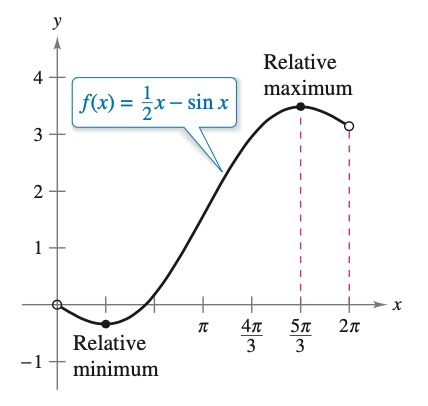
\includegraphics[width=0.55\linewidth]{Example_27.jpg} % Adjust the image width as necessary
    \captionof{figure}{}
    \label{fig:graph}
\end{minipage}
\end{tcolorbox}


\begin{tcolorbox}[colback=examplebg, colframe=red!75!black, title=\textbf{EXAMPLE 2: Applying the First Derivative Test}, fonttitle=\bfseries, sharp corners]
Find the relative extrema of \( f(x) = \frac{x^4 + 1}{x^2} \).
\tcblower
\textbf{Solution:} 
\quad Note that \( f \) is not defined when \( x = 0 \).

\[
f(x) = x^2 + x^{-2} \quad \text{\textit{Rewrite original function.}}
\]
\[
f'(x) = 2x - 2x^{-3} \quad \text{\textit{Differentiate.}}
\]
\[
= 2x - \frac{2}{x^3} \quad \text{\textit{Rewrite with positive exponent.}}
\]
\[
= \frac{2(x^4 - 1)}{x^3} \quad \text{\textit{Simplify.}}
\]
\[
= \frac{2(x^2 + 1)(x - 1)(x + 1)}{x^3} \quad \text{\textit{Factor.}}
\]

So, \( f'(x) \) is zero at \( x = \pm 1 \). Moreover, because \( x = 0 \) is not in the domain of \( f \), you should use this \( x \)-value along with the critical numbers to determine the test intervals.
\[
x = \pm 1 \quad x = 0 \quad \text{\textit{Critical numbers, \( f'(\pm 1) = 0 \)}}.
\]
\[
\text{\textit{0 is not in the domain of \( f \).}}
\]


\[
\begin{array}{|c|c|c|c|c|}
\hline
\textbf{Interval} & -\infty < x < -1 & -1 < x < 0 & 0 < x < 1 & 1 < x < \infty \\
\hline
\textbf{Test Value} & x = -2 & x = -\frac{1}{2} & x = \frac{1}{2} & x = 2 \\
\hline
\textbf{Sign of \( f'(x) \)} & f'(-2) < 0 & f'\left( -\frac{1}{2} \right) > 0 & f'\left( \frac{1}{2} \right) < 0 & f'(2) > 0 \\
\hline
\textbf{Conclusion} & \text{Decreasing} & \text{Increasing} & \text{Decreasing} & \text{Increasing} \\
\hline
\end{array}
\]

\begin{minipage}{\linewidth}
    \centering
    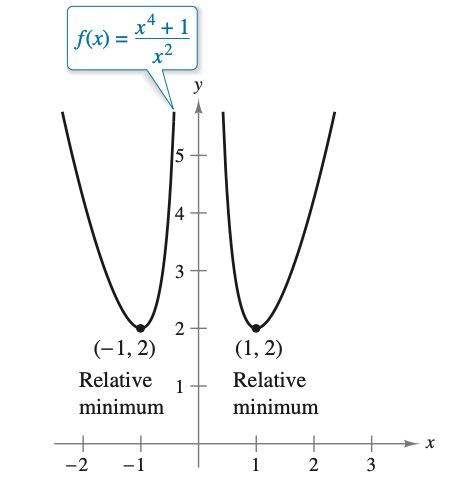
\includegraphics[width=0.49\linewidth]{Example_28.jpg} % Adjust the image width as necessary
    \captionof{figure}{}
    \label{fig:graph}
\end{minipage}
\end{tcolorbox}

\subsection{Determine Absolute Extrema from Candidates}
\begin{Note}{Determining Absolute Extrema from Candidates}{}
\vspace{2mm}
\noindent
Let \( f \) be a \textbf{continuous} function on a \textbf{closed interval} \( [a, b] \). To determine the \textbf{absolute maximum} and \textbf{absolute minimum} values of \( f \) on \( [a, b] \), follow these steps:

\begin{enumerate}
    \item \textbf{Find the critical numbers:} Solve \( f'(x) = 0 \) or determine where \( f'(x) \) does not exist in the open interval \( (a, b) \).
    \item \textbf{Evaluate the function:} Calculate \( f(x) \) at:
    \begin{itemize}
        \item \textbf{The critical numbers} found in Step 1, and
        \item \textbf{The endpoints} \( x = a \) and \( x = b \).
    \end{itemize}
    \item \textbf{Compare values:} The largest value of \( f(x) \) is the \textbf{\color{red}absolute maximum}, and the smallest value of \( f(x) \) is the \textbf{\color{blue}absolute minimum}.
\end{enumerate}
\vspace{3mm}
\noindent
\textit{\textbf{Important Note:}} The continuity of \( f \) on the closed interval \( [a, b] \) is \textbf{essential} for this method to guarantee the existence of absolute extrema.
\end{Note}

\begin{tcolorbox}[colback=examplebg, colframe=red!75!black, title=\textbf{EXAMPLE 1: Find the Absolute Value}, fonttitle=\bfseries, sharp corners]
Find the absolute maximum value and the absolute minimum value of the function
\[
f(x) = x^3 - 3x^2 + 1 \quad \text{on the interval} \quad \left[ -\frac{1}{2}, 4 \right].
\]
\tcblower
\textbf{Solution:} 
\vspace{2mm}

\textbf{Step 1: Find the derivative of \( f(x) \).}

\[
f'(x) = 3x^2 - 6x.
\]

\textbf{Step 2: Solve \( f'(x) = 0 \) to find critical points.}

\[
3x^2 - 6x = 0.
\]
Factor out \( 3x \):
\[
3x(x - 2) = 0 \implies x = 0 \ \text{or} \ x = 2.
\]

\textbf{Step 3: Evaluate \( f(x) \) at the critical points and the endpoints \( x = -\frac{1}{2} \) and \( x = 4 \).}

\[
f(x) = x^3 - 3x^2 + 1.
\]
\begin{itemize}
    \item At \( x = -\frac{1}{2} \):
    \[
    f\left( -\frac{1}{2} \right) = \left( -\frac{1}{2} \right)^3 - 3\left( -\frac{1}{2} \right)^2 + 1 = -\frac{1}{8} - \frac{3}{4} + 1 = \frac{1}{8}.
    \]

    \item At \( x = 0 \):
    \[
    f(0) = 0^3 - 3(0)^2 + 1 = 1.
    \]

    \item At \( x = 2 \):
    \[
    f(2) = 2^3 - 3(2)^2 + 1 = 8 - 12 + 1 = -3.
    \]

    \item At \( x = 4 \):
    \[
    f(4) = 4^3 - 3(4)^2 + 1 = 64 - 48 + 1 = 17.
    \]
\end{itemize}

\textbf{Step 4: Compare the values of \( f(x) \).}

The values are:
\[
f\left( -\frac{1}{2} \right) = \frac{1}{8}, \quad f(0) = 1, \quad f(2) = -3, \quad f(4) = 17.
\]

\textbf{Conclusion:}

\begin{itemize}
    \item The \textbf{absolute maximum} value is \( 17 \) at \( x = 4 \).
    \item The \textbf{absolute minimum} value is \( -3 \) at \( x = 2 \).
\end{itemize}
\end{tcolorbox}

\subsection{Concavity and the Second Derivative Test}
\subsubsection{Concavity}
\begin{Definition}{Concavity}
\noindent
Let \( f \) be differentiable on an open interval \( I \). The graph of \( f \) is \textbf{concave upward} on \( I \) when \( f' \) is increasing on the interval and \textbf{concave downward} on \( I \) when \( f' \) is decreasing on the interval.   
\end{Definition}
\begin{minipage}{\linewidth}
    \centering
    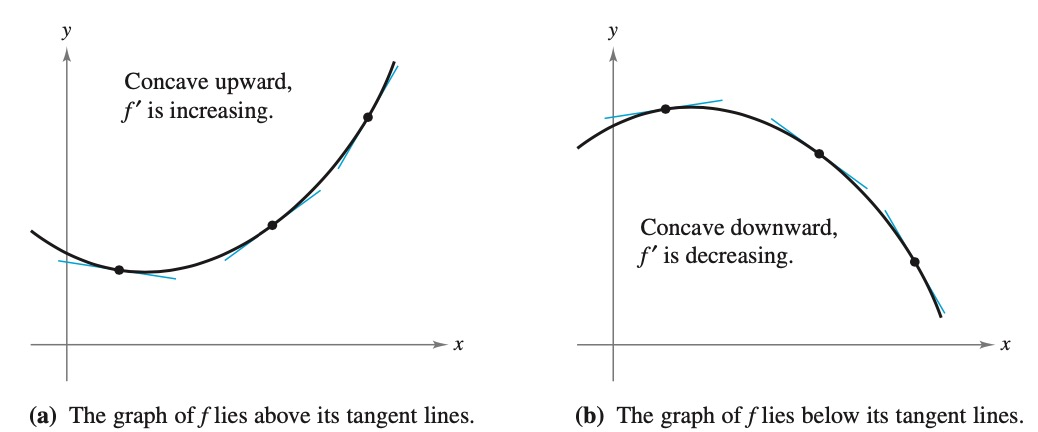
\includegraphics[width=0.80\linewidth]{Example_29.jpg} % Adjust the image width as necessary
    \captionof{figure}{}
    \label{fig:graph}
\end{minipage}

\begin{mytheorem}{Test for Concavity}
\noindent
Let \( f \) be a function whose second derivative exists on an open interval \( I \).

\begin{enumerate}
    \item If \( f''(x) > 0 \) for all \( x \) in \( I \), then the graph of \( f \) is concave upward on \( I \).
    \item If \( f''(x) < 0 \) for all \( x \) in \( I \), then the graph of \( f \) is concave downward on \( I \).
\end{enumerate}
\end{mytheorem}


\begin{tcolorbox}[colback=examplebg, colframe=red!75!black, title=\textbf{EXAMPLE 1: Determining Concavity}, fonttitle=\bfseries, sharp corners]
\noindent
Determine the open intervals on which the graph of
\[
f(x) = \frac{6}{x^2 + 3}
\]
is concave upward or downward.
\tcblower
\textbf{Solution:} 
\quad Begin by observing that \( f \) is continuous on the entire real number line. Next, find the second derivative of \( f \).

\[
f(x) = 6(x^2 + 3)^{-1} \quad \text{\textit{Rewrite original function.}}
\]
\[
f'(x) = (-6)(x^2 + 3)^{-2}(2x) \quad \text{\textit{Differentiate.}}
\]
\[
= \frac{-12x}{(x^2 + 3)^2} \quad \text{\textit{First derivative.}}
\]
\[
f''(x) = \frac{(x^2 + 3)^2(-12) - (-12x)(2)(x^2 + 3)(2x)}{(x^2 + 3)^4} \quad \text{\textit{Differentiate.}}
\]
\[
= \frac{36(x^2 - 1)}{(x^2 + 3)^3} \quad \text{\textit{Second derivative.}}
\]

Because \( f''(x) = 0 \) when \( x = \pm 1 \) and \( f'' \) is defined on the entire real number line, you should test \( f'' \) in the intervals \( (-\infty, -1) \), \( (-1, 1) \), and \( (1, \infty) \). The results are shown in the table below.

\vspace{3mm}

\[
\begin{array}{|c|c|c|c|}
\hline
\textbf{Interval} & -\infty < x < -1 & -1 < x < 1 & 1 < x < \infty \\
\hline
\textbf{Test Value} & x = -2 & x = 0 & x = 2 \\
\hline
\textbf{Sign of \( f''(x) \)} & f''(-2) > 0 & f''(0) < 0 & f''(2) > 0 \\
\hline
\textbf{Conclusion} & \text{Concave upward} & \text{Concave downward} & \text{Concave upward} \\
\hline
\end{array}
\]

\end{tcolorbox}
\newpage
\subsubsection{Points of Inflection}
\begin{Definition}{Point of Inflection}
\noindent
Let \( f \) be a function that is continuous on an open interval, and let \( c \) be a point in the interval. If the graph of \( f \) has a tangent line at this point \( (c, f(c)) \), then this point is a \textbf{point of inflection} of the graph of \( f \) when the concavity of \( f \) changes from upward to downward (or downward to upward) at the point.
\end{Definition}
\noindent
\begin{minipage}{0.5\linewidth}
    \centering
    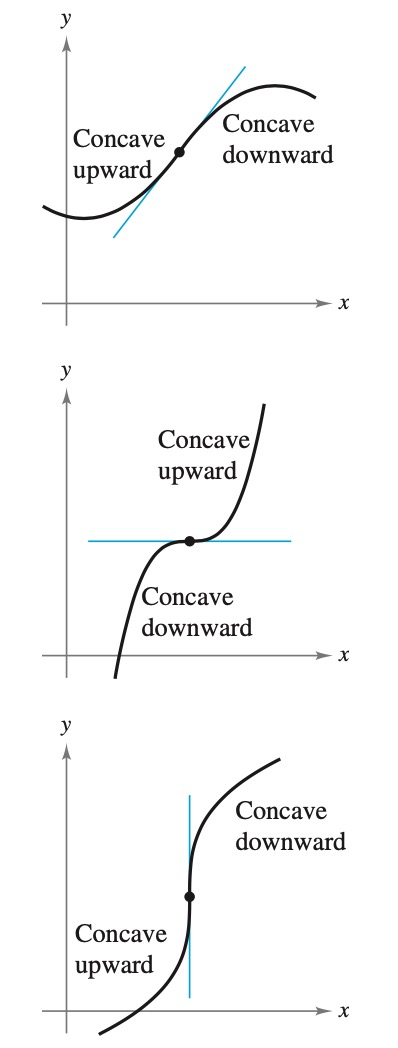
\includegraphics[width=0.55\linewidth]{Example_30.jpg} % 替换为你的图片路径
    \captionof{figure}{Concavity and Points of Inflection}
    \label{fig:graph}
\end{minipage}%
\hspace{5mm} % 增加间距
\begin{minipage}{0.55\linewidth}
    \noindent
    At a \textbf{point of inflection}:
    \begin{itemize}
        \item The concavity of the graph changes.
        \item Either \( f''(c) = 0 \) or \( f'' \) does not exist.
        \item Tangent lines can still exist, as shown in the figure.
    \end{itemize}
\end{minipage}

\begin{mytheorem}{Points of Inflection}
\noindent
If \( (c, f(c)) \) is a point of inflection of the graph of \( f \), then either \( f''(c) = 0 \) or \( f'' \) does not exist at \( x = c \).
\end{mytheorem}

\begin{tcolorbox}[colback=examplebg, colframe=red!75!black, title=\textbf{EXAMPLE 2: Finding Points of Inflection}, fonttitle=\bfseries, sharp corners]
Determine the points of inflection and discuss the concavity of the graph of
\[
f(x) = x^4 - 4x^3.
\]

\tcblower
\textbf{Solution:} 
\quad Differentiating twice produces the following:
\[
f(x) = x^4 - 4x^3 \quad \text{\textit{Write original function.}}
\]
\[
f'(x) = 4x^3 - 12x^2 \quad \text{\textit{Find first derivative.}}
\]
\[
f''(x) = 12x^2 - 24x = 12x(x - 2) \quad \text{\textit{Find second derivative.}}
\]

\noindent
Setting \( f''(x) = 0 \), you can determine that the possible points of inflection occur at \( x = 0 \) and \( x = 2 \). By testing the intervals determined by these \( x \)-values, you can conclude that they both yield points of inflection. A summary of this testing is shown in the table below.

\vspace{3mm}

\noindent
\[
\begin{array}{|c|c|c|c|}
\hline
\textbf{Interval} & -\infty < x < 0 & 0 < x < 2 & 2 < x < \infty \\
\hline
\textbf{Test Value} & x = -1 & x = 1 & x = 3 \\
\hline
\textbf{Sign of \( f''(x) \)} & f''(-1) > 0 & f''(1) < 0 & f''(3) > 0 \\
\hline
\textbf{Conclusion} & \text{Concave upward} & \text{Concave downward} & \text{Concave upward} \\
\hline
\end{array}
\]
\begin{minipage}{\linewidth}
    \centering
    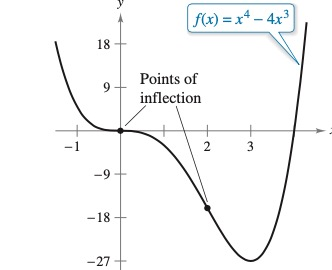
\includegraphics[width=0.60\linewidth]{Example_31.jpg} % Adjust the image width as necessary
    \captionof{figure}{}
    \label{fig:graph}
\end{minipage}
\end{tcolorbox}
\newpage

\subsubsection{The Second Derivative Test}
\begin{mytheorem}{Second Derivative Test}{}
\noindent
Let \( f \) be a function such that \( f'(c) = 0 \) and the second derivative of \( f \) exists on an open interval containing \( c \).

\begin{enumerate}
    \item If \( f''(c) > 0 \), then \( f \) has a \textit{relative minimum} at \( (c, f(c)) \).
    \item If \( f''(c) < 0 \), then \( f \) has a \textit{relative maximum} at \( (c, f(c)) \).
\end{enumerate}

\noindent
If \( f''(c) = 0 \), then the test fails. That is, \( f \) may have a relative maximum, a relative minimum, or neither. In such cases, you can use the \textit{First Derivative Test}.
\end{mytheorem}

\begin{tcolorbox}[colback=examplebg, colframe=red!75!black, title=\textbf{EXAMPLE 3: Using the Second Derivative Test}, fonttitle=\bfseries, sharp corners]
\noindent
Find the relative extrema of 
\[
f(x) = -3x^5 + 5x^3.
\]

\noindent

\tcblower
\textbf{Solution:}
\quad Begin by finding the first derivative of \( f \):
\[
f'(x) = -15x^4 + 15x^2 = 15x^2(1 - x^2).
\]
From this derivative, you can see that \( x = -1, 0, \) and \( 1 \) are the only critical numbers of \( f \). By finding the second derivative:
\[
f''(x) = -60x^3 + 30x = 30x(1 - 2x^2),
\]
you can apply the Second Derivative Test as shown below.

\vspace{3mm}
\noindent
\[
\begin{array}{|c|c|c|c|}
\hline
\textbf{Point} & (-1, -2) & (0, 0) & (1, 2) \\
\hline
\textbf{Sign of \( f''(x) \)} & f''(-1) > 0 & f''(0) = 0 & f''(1) < 0 \\
\hline
\textbf{Conclusion} & \text{Relative minimum} & \text{Test fails} & \text{Relative maximum} \\
\hline
\end{array}
\]

\begin{minipage}{\linewidth}
    \centering
    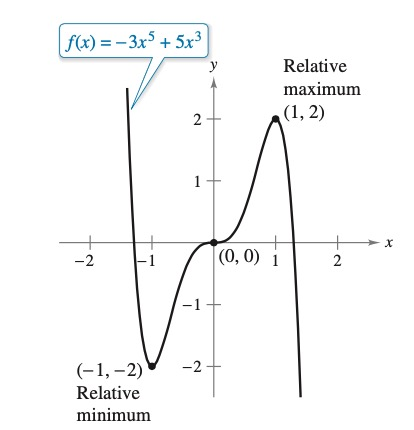
\includegraphics[width=0.35\linewidth]{Example_32.jpg} % Adjust the image width as necessary
    \captionof{figure}{}
    \label{fig:graph}
\end{minipage}
\end{tcolorbox}

\subsection{Sketching Graphs of Functions and Their Derivatives }
\begin{Note}{Guidelines for Sketching a Curve}
\noindent The following checklist summarizes the main steps for sketching a curve \( y = f(x) \):
\begin{enumerate} % Main list with custom labels
    \item \textbf{Domain:} Determine the domain \( D \) of \( f \), i.e., the set of \( x \)-values for which \( f(x) \) is defined.

    \item \textbf{Intercepts:} Find where the curve intersects the axes. The \( y \)-intercept is \( f(0) \), and the \( x \)-intercepts satisfy \( y = 0 \).

    \item \textbf{Symmetry:} 
    \begin{enumerate}
        \item If \( f(-x) = f(x) \), the curve is symmetric about the \( y \)-axis (\textit{even function}).
        \item If \( f(-x) = -f(x) \), the curve is symmetric about the origin (\textit{odd function}).
        \item If \( f(x + p) = f(x) \), the curve is periodic with period \( p \).
    \end{enumerate}

    \item \textbf{Asymptotes:} 
    \begin{enumerate}
        \item \textit{Horizontal Asymptotes:} Check the limits as \( x \to \infty \) and \( x \to -\infty \).
        \item \textit{Vertical Asymptotes:} Identify where the function diverges, such as when the denominator equals zero.
        \item \textit{Slant Asymptotes:} Analyze the behavior for large \( |x| \) if horizontal asymptotes do not exist.
    \end{enumerate}

    \item \textbf{Intervals of Increase or Decrease:} Use \( f'(x) \) to find where the curve is increasing (\( f'(x) > 0 \)) or decreasing (\( f'(x) < 0 \)).

    \item \textbf{Local Maximum or Minimum Values:} Find critical points by setting \( f'(x) = 0 \) or identifying where \( f'(x) \) does not exist. Use the First or Second Derivative Test to classify extrema.

    \item \textbf{Concavity and Points of Inflection:} Compute \( f''(x) \). If \( f''(x) > 0 \), the curve is concave upward; if \( f''(x) < 0 \), it is concave downward. Points of inflection occur where \( f''(x) = 0 \) or \( f''(x) \) does not exist.

    \item \textbf{Sketch the Curve:} Combine all the information (A--G) to sketch the curve, including key features like intercepts, symmetry, asymptotes, intervals of increase/decrease, and points of inflection.
\end{enumerate}
\end{Note}


\begin{tcolorbox}[colback=examplebg, colframe=red!75!black, title=\textbf{EXAMPLE 1:Sketching the Curve}, fonttitle=\bfseries, sharp corners]
\noindent Use the guidelines to sketch the curve \( y = \frac{-2x^2}{x^2 - 1} \).

\tcblower
\textbf{Solution:} 
\begin{enumerate}
    \item \textbf{Domain:} 
    \[
    \{ x \mid x^2 - 1 \neq 0 \} = \{ x \mid x \neq \pm 1 \} = (-\infty, -1) \cup (-1, 1) \cup (1, \infty).
    \]

    \item \textbf{Intercepts:} 
    The \( x \)- and \( y \)-intercepts are both \( 0 \).

    \item \textbf{Symmetry:} 
    Since \( f(-x) = f(x) \), \( f \) is even and symmetric about the \( y \)-axis.

    \item \textbf{Asymptotes:}
    \begin{itemize}
        \item Horizontal: \( \lim_{x \to \pm \infty} \frac{2x^2}{x^2 - 1} = 2 \Rightarrow y = 2 \).
        \item Vertical: At \( x = \pm 1 \), \( \lim_{x \to 1^{+}} \to \infty \) and \( \lim_{x \to 1^{-}} \to -\infty \), so \( x = \pm 1 \) are vertical asymptotes.
    \end{itemize}

    \item \textbf{Intervals of Increase or Decrease:}
    \[
    f'(x) = \frac{-4x}{(x^2 - 1)^2}.
    \]
    \( f'(x) > 0 \) when \( x < 0 \) (excluding \( x = -1 \)) and \( f'(x) < 0 \) when \( x > 0 \) (excluding \( x = 1 \)).

    \item \textbf{Local Maximum or Minimum Values:}
    \( x = 0 \) is the only critical point. Since \( f'(x) \) changes sign at \( x = 0 \), \( f(0) = 0 \) is a local maximum.

    \item \textbf{Concavity and Points of Inflection:}
    \[
    f''(x) = \frac{12x^2 + 4}{(x^2 - 1)^3}.
    \]
    \( f''(x) > 0 \) when \( |x| > 1 \) (concave upward), and \( f''(x) < 0 \) when \( |x| < 1 \) (concave downward).

    \item \textbf{Sketch the Curve:}
    Combine all information: domain, intercepts, symmetry, asymptotes, intervals of increase/decrease, and concavity.
\end{enumerate}
\begin{minipage}{\linewidth}
    \centering
    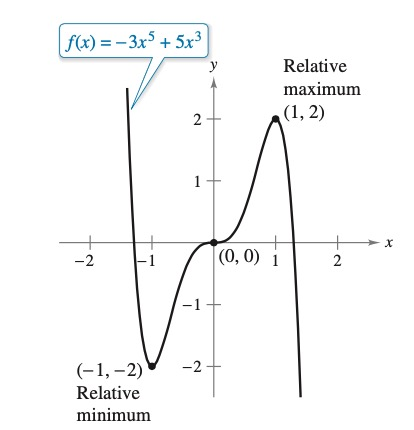
\includegraphics[width=0.20\linewidth]{Example_32.jpg} % Adjust the image width as necessary
\end{minipage}
\end{tcolorbox}



\begin{tcolorbox}[colback=examplebg, colframe=red!75!black, title=\textbf{EXAMPLE 2: Sketching the Curve: Tangent Line Approximation}, fonttitle=\bfseries, sharp corners]
\noindent Use the guidelines to sketch the curve \( y = \frac{-2x^2}{x^2 - 1} \).
\tcblower
\textbf{Solution:} 
\begin{enumerate}
    \item \textbf{Domain:} 
    \[
    \{ x \mid x^2 - 1 \neq 0 \} = \{ x \mid x \neq \pm 1 \} = (-\infty, -1) \cup (-1, 1) \cup (1, \infty).
    \]

    \item \textbf{Intercepts:} 
    The \( x \)- and \( y \)-intercepts are both \( 0 \).

    \item \textbf{Symmetry:} 
    Since \( f(-x) = f(x) \), \( f \) is even and symmetric about the \( y \)-axis.

    \item \textbf{Asymptotes:}
    \begin{itemize}
        \item Horizontal: \( \lim_{x \to \pm \infty} \frac{2x^2}{x^2 - 1} = 2 \Rightarrow y = 2 \).
        \item Vertical: At \( x = \pm 1 \), \( \lim_{x \to 1^{+}} \to \infty \) and \( \lim_{x \to 1^{-}} \to -\infty \), so \( x = \pm 1 \) are vertical asymptotes.
    \end{itemize}

    \item \textbf{Intervals of Increase or Decrease:}
    \[
    f'(x) = \frac{-4x}{(x^2 - 1)^2}.
    \]
    \( f'(x) > 0 \) when \( x < 0 \) (excluding \( x = -1 \)) and \( f'(x) < 0 \) when \( x > 0 \) (excluding \( x = 1 \)).

    \item \textbf{Local Maximum or Minimum Values:}
    \( x = 0 \) is the only critical point. Since \( f'(x) \) changes sign at \( x = 0 \), \( f(0) = 0 \) is a local maximum.

    \item \textbf{Concavity and Points of Inflection:}
    \[
    f''(x) = \frac{12x^2 + 4}{(x^2 - 1)^3}.
    \]
    \( f''(x) > 0 \) when \( |x| > 1 \) (concave upward), and \( f''(x) < 0 \) when \( |x| < 1 \) (concave downward).

    \item \textbf{Sketch the Curve:}
    Combine all information: domain, intercepts, symmetry, asymptotes, intervals of increase/decrease, and concavity.
\end{enumerate}

\begin{minipage}{\linewidth}
    \centering
    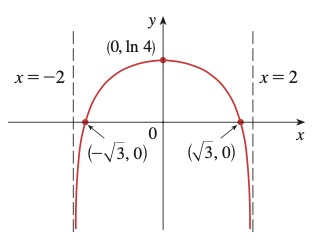
\includegraphics[width=0.29\linewidth]{Example_34.jpg} % Adjust the image width as
\end{minipage}
\end{tcolorbox}

\subsection{Connecting a Function, Its 1st, and its 2nd Derivative}
\noindent\textbf{\textcolor{blue}{Key Concept:}}  
\begin{tcolorbox}[colback=blue!10, colframe=blue!30, title=Main Concept]
The \textbf{first derivative} tells you where the original function is increasing or decreasing, based on its positive or negative value:
\begin{itemize}
    \item \textbf{\textcolor{green!50!black}{Positive value:}} Function is \textbf{increasing}.
    \item \textbf{\textcolor{red}{Negative value:}} Function is \textbf{decreasing}.
    \item \textbf{\textcolor{orange!70!black}{Zero value:}} Potential \textbf{maximum or minimum point}.
\end{itemize}

The \textbf{second derivative} indicates the concavity of the function:  
\begin{itemize}
    \item \textcolor{green!50!black}{Positive second derivative:} Concave up (curving upwards).  
    \item \textcolor{red}{Negative second derivative:} Concave down (curving downwards).  
    \item \textbf{\textcolor{orange!70!black}{Zero value:}} Potential \textbf{inflection point} where concavity changes.
\end{itemize}
\end{tcolorbox}

\noindent\textbf{\textcolor{blue}{Key Points to Remember:}} 

\vspace{5pt}

\begin{array}{|l|c|l|}
\hline
f'(x) > 0 & \to & f(x) \, \text{is increasing} \\ \hline
f'(x) < 0 & \to & f(x) \, \text{is decreasing} \\ \hline
f'(x) \, \text{changes from negative to positive} & \to & f(x) \, \text{has a relative minimum} \\ \hline
f'(x) \, \text{changes from positive to negative} & \to & f(x) \, \text{has a relative maximum} \\ \hline
f'(x) \, \text{is increasing} & \to & f(x) \, \text{is concave upward} \\ \hline
f'(x) \, \text{is decreasing} & \to & f(x) \, \text{is concave downward} \\ \hline
f'(x) \, \text{has an extreme value} & \to & f(x) \, \text{has a point of inflection} \\ \hline
\end{array}
\]

\vspace{5pt}

\begin{minipage}{\linewidth}
    \centering
    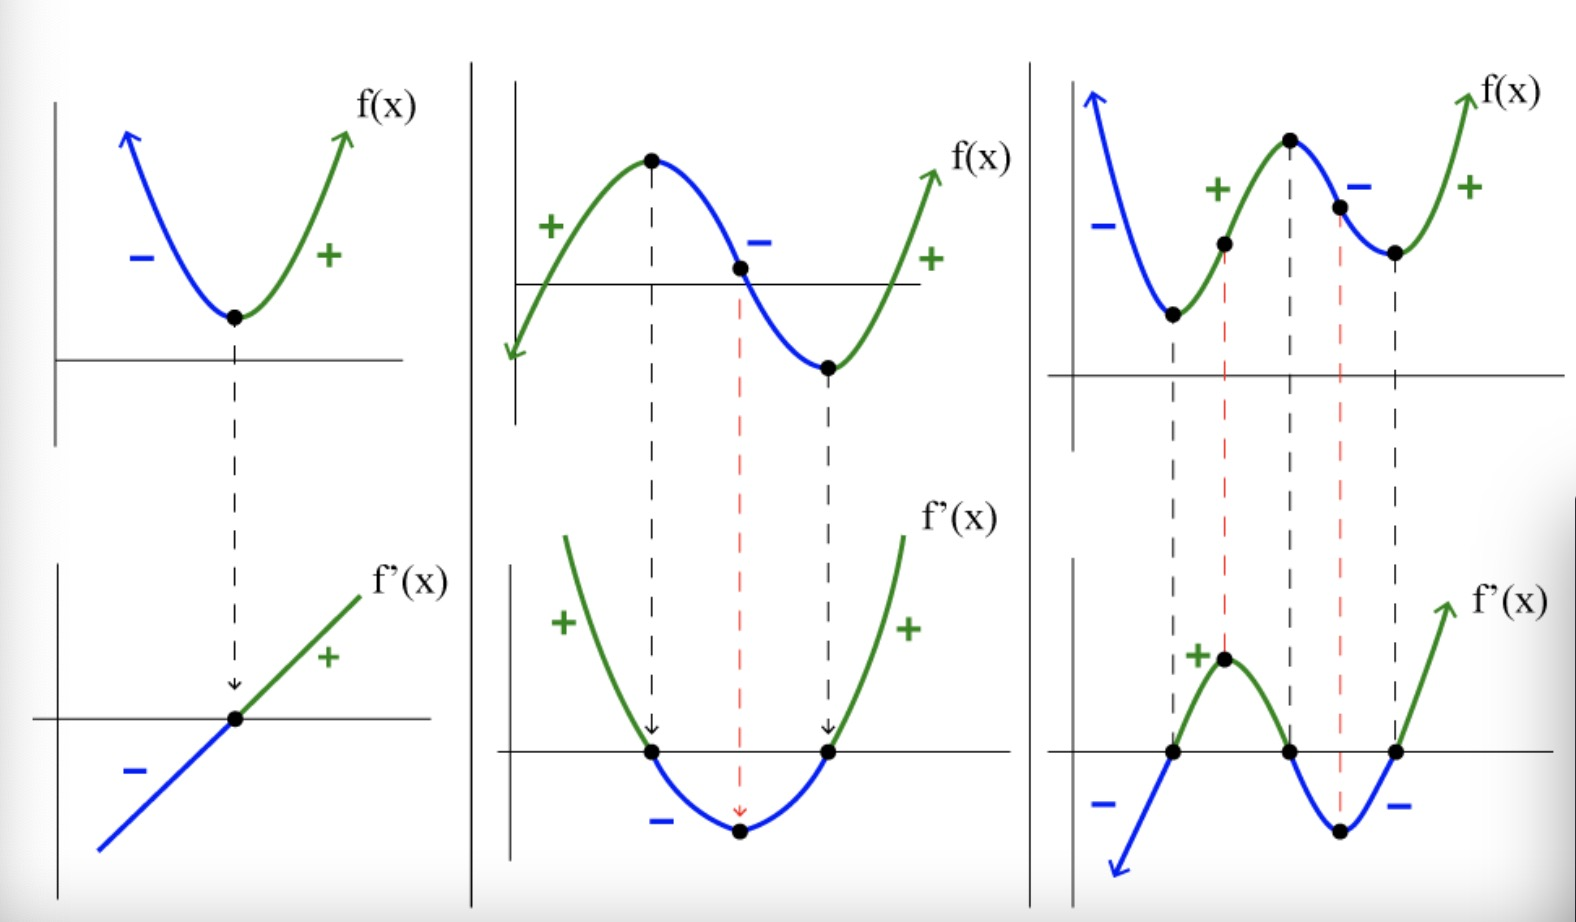
\includegraphics[width=0.80\linewidth]{Example_35.jpg} % Adjust the image width as
\end{minipage}



\begin{tcolorbox}[colback=examplebg, colframe=red!75!black, title=\textbf{EXAMPLE 1: Determine Which is Which}, fonttitle=\bfseries, sharp corners]

The graph displays three curves: a function \( f \), its first derivative \( f' \), and its second derivative \( f'' \). We can determine which curve is which by analyzing the following behaviors:

\begin{minipage}{\linewidth}
    \centering
    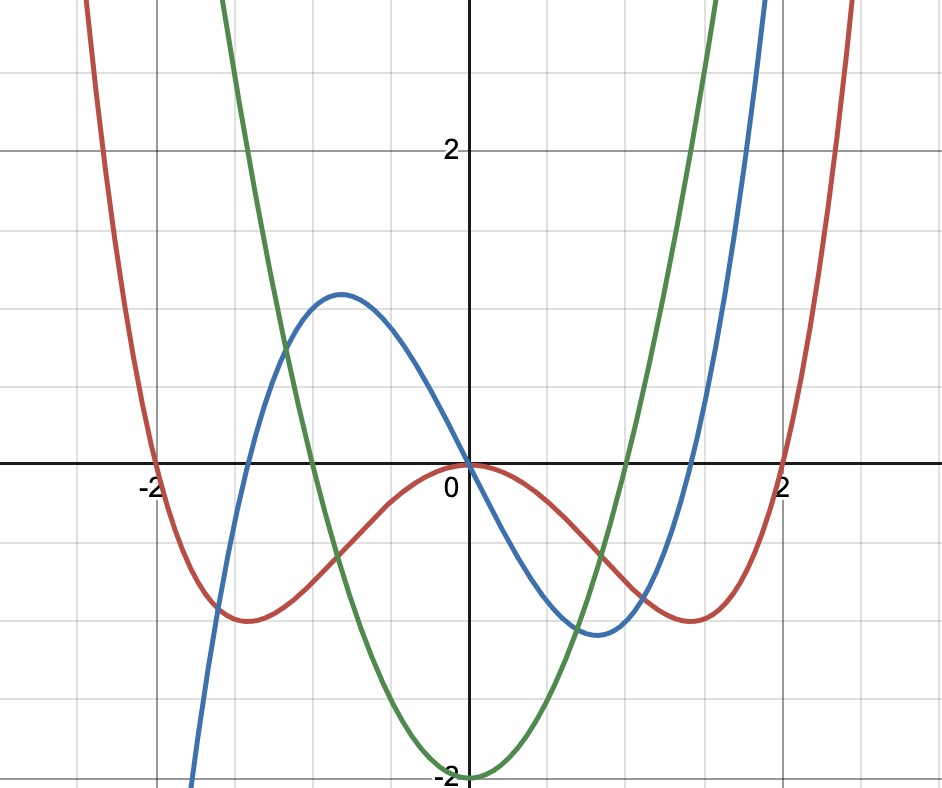
\includegraphics[width=0.40\linewidth]{Example_36.jpg} % Adjust the image width as
\end{minipage}
\tcblower
\textbf{Solution:} 
The graph displays three curves: a function \( f \), its first derivative \( f' \), and its second derivative \( f'' \). We can determine which curve is which by analyzing the following behaviors:

\begin{enumerate}
    \item \textbf{Behavior of the function \( f \):}
    \begin{itemize}
        \item \( f \) has \textbf{critical points} (local minima or maxima) where \( f'(x) = 0 \), i.e., where the derivative curve crosses the \( x \)-axis.
        \item \( f \) is \textbf{concave up} where \( f''(x) > 0 \) and \textbf{concave down} where \( f''(x) < 0 \).
    \end{itemize}

    \item \textbf{Behavior of the first derivative \( f' \):}
    \begin{itemize}
        \item \( f' \) has \textbf{zeros} where \( f \) has local extrema.
        \item \( f' \) is increasing where \( f'' > 0 \) and decreasing where \( f'' < 0 \).
    \end{itemize}

    \item \textbf{Behavior of the second derivative \( f'' \):}
    \begin{itemize}
        \item \( f'' \) crosses the \( x \)-axis where \( f' \) has critical points (maxima or minima).
        \item \( f'' \) determines the concavity of \( f \): positive values mean \( f \) is concave up, and negative values mean \( f \) is concave down.
    \end{itemize}
\end{enumerate}

\noindent\textbf{Identifying the Curves:}
\begin{itemize}
    \item The \textbf{blue curve} represents \( f \), as it shows local maxima and minima (the original function).
    \item The \textbf{red curve} represents \( f' \), as it crosses the \( x \)-axis where \( f \) has critical points.
    \item The \textbf{green curve} represents \( f'' \), as it crosses the \( x \)-axis where \( f' \) has critical points and determines concavity.
\end{itemize}




\end{tcolorbox}

\subsection{Optimization Problems}
\subsubsection{Introduction to Optimization Problems}
\begin{Definition}{Optimization }
\textbf{Optimization} is the process of making something the \textbf{best it can possibly be} under given constraints.
\end{Definition}

\vspace{5mm}

\noindent\textbf{\textcolor{blue}{A Classic Optimization Problem}}

\noindent You want to enclose a garden with fencing to keep rabbits away. A shed serves as the boundary for one side, and fencing is needed for the other three sides. Given \textbf{60 feet of fencing}, what is the area of the \textbf{largest garden} you can enclose?

\vspace{3mm}

\noindent\textbf{\textcolor{green!50!black}{Steps to Solve:}}

\begin{enumerate}
    \item \textbf{\textcolor{black}{Write an equation:}} Identify the area to be maximized.
    \item \textbf{\textcolor{black}{Use constraints:}} Use the fencing length to form relationships between the sides.
    \item \textbf{\textcolor{black}{Rewrite the equation:}} Express the area equation using one variable.
    \item \textbf{\textcolor{black}{Find critical values:}} Use derivatives to find the maximum area.
    \item \textbf{\textcolor{black}{Interpret the result:}} State the maximum area clearly and in context.
\end{enumerate}

\subsubsection{Optimization Problems}
\begin{tcolorbox}[colback=examplebg, colframe=red!75!black, title=\textbf{Example 1: Finding Maximum Volume}, fonttitle=\bfseries, sharp corners]
A manufacturer wants to design an open box with a square base and a surface area of \( 108 \, \text{in}^2 \). What dimensions will produce a box with maximum volume?

\begin{minipage}{\linewidth}
    \centering
    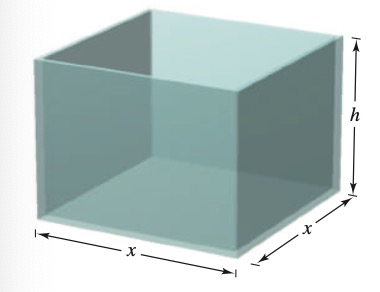
\includegraphics[width=0.30\linewidth]{Example_37.jpg} % Adjust the image width as
\end{minipage}

\tcblower
\textbf{Solution:} 
\begin{enumerate}
    \item \textbf{Primary Equation:}  
    The volume of the box is:
    \[
    V = x^2 h \quad \text{(square base with height \( h \))}.
    \]

    \item \textbf{Secondary Equation:}  
    From the surface area constraint:
    \[
    x^2 + 4xh = 108 \implies h = \frac{108 - x^2}{4x}.
    \]

    \item \textbf{Simplify \( V \):}  
    Substitute \( h \) into \( V \):
    \[
    V = x^2 \left( \frac{108 - x^2}{4x} \right) = 27x - \frac{x^3}{4}.
    \]

    \item \textbf{Feasible Domain:}  
    \( V \geq 0 \) and the area constraint gives:
    \[
    0 \leq x \leq \sqrt{108}.
    \]

    \item \textbf{Differentiate to Find Critical Numbers:}  
    \[
    \frac{dV}{dx} = 27 - \frac{3x^2}{4}.
    \]
    Set \( \frac{dV}{dx} = 0 \):
    \[
    27 - \frac{3x^2}{4} = 0 \implies x^2 = 36 \implies x = 6 \, (\text{since } x > 0).
    \]

    \item \textbf{Evaluate \( V \):}  
    Evaluate \( V \) at critical points and endpoints:
    \[
    V(0) = 0, \quad V(6) = 108, \quad V(\sqrt{108}) = 0.
    \]
    The maximum volume is \( V = 108 \, \text{in}^3 \) at \( x = 6 \) inches.

\end{enumerate}

\end{tcolorbox}


\begin{tcolorbox}[colback=examplebg, colframe=red!75!black, title=\textbf{Example 2: Finding Minimum Distance}, fonttitle=\bfseries, sharp corners]
Find the points on the graph \( y = 4 - x^2 \) that are closest to the point \( (0, 2) \).



\begin{minipage}{\linewidth}
    \centering
    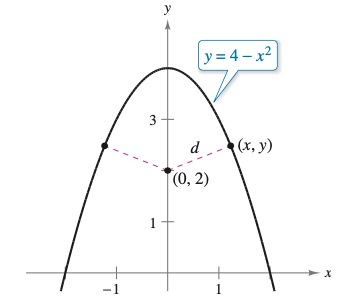
\includegraphics[width=0.30\linewidth]{Example_38.jpg} % Adjust the image width as
\end{minipage}

\tcblower
\textbf{Solution:} 

\begin{enumerate}
    \item \textbf{Primary Equation:}  
    The distance \( d \) between \( (0, 2) \) and a point \( (x, y) \) on the curve is:
    \[
    d = \sqrt{(x - 0)^2 + (y - 2)^2}.
    \]

    \item \textbf{Substitute \( y = 4 - x^2 \):}  
    Rewrite \( d \) as:
    \[
    d = \sqrt{x^2 + (4 - x^2 - 2)^2} = \sqrt{x^4 - 3x^2 + 4}.
    \]

    \item \textbf{Find Critical Points:}  
    Minimize \( f(x) = x^4 - 3x^2 + 4 \) by differentiating:
    \[
    f'(x) = 4x^3 - 6x = 2x(2x^2 - 3).
    \]
    Setting \( f'(x) = 0 \), we get:
    \[
    x = 0, \quad x = \pm \sqrt{\frac{3}{2}}.
    \]

    \item \textbf{Test Critical Points:}  
    Using the First Derivative Test:
    \begin{itemize}
        \item \( x = 0 \): Yields a relative maximum.
        \item \( x = \pm \sqrt{3/2} \): Yield minimum distances.
    \end{itemize}

    \item \textbf{Closest Points:}  
    Substitute \( x = \pm \sqrt{3/2} \) into \( y = 4 - x^2 \):
    \[
    y = 4 - \left( \frac{3}{2} \right) = \frac{5}{2}.
    \]
    The closest points are:
    \[
    \left( \sqrt{\frac{3}{2}}, \frac{5}{2} \right) \quad \text{and} \quad \left( -\sqrt{\frac{3}{2}}, \frac{5}{2} \right).
    \]
\end{enumerate}



\end{tcolorbox}

\subsection{Exploring Behaviors of Implicit Relations}

\begin{Note}{Connections Between the derivative}
\noindent\textbf{\textcolor{purple}{Implicit Differentiation:}}
Differentiate both sides of the equation \( F(x, y) = 0 \) with respect to \( x \), treating \( y \) as a function of \( x \). 
\vspace{5pt}

\noindent\textbf{\textcolor{red}{Slope of the Tangent Line:}}  
The derivative \( \frac{dy}{dx} \) represents the slope of the tangent line to the curve at any point \( (x, y) \).

\vspace{5pt}

\noindent\textbf{\textcolor{orange}{Horizontal and Vertical Tangents:}}  
\begin{itemize}
    \item \textbf{Horizontal tangent:} \( \frac{dy}{dx} = 0 \) occurs when \( F_x = 0 \) and \( F_y \neq 0 \).
    \item \textbf{Vertical tangent:} \( \frac{dy}{dx} \to \infty \) occurs when \( F_y = 0 \) and \( F_x \neq 0 \).
\end{itemize}
\end{Note}

\begin{tcolorbox}[colback=examplebg, colframe=red!75!black, title=\textbf{EXAMPLE 1:Differentiate the given implicit equation}, fonttitle=\bfseries, sharp corners]
\noindent Show that $\frac{dy}{dx} = \frac{2y - 4x - 4}{y - 2x}$ for the graph $4x^2 - 4xy + y^2 + 8x = 12$.\\
\tcblower
\textbf{Solution:} 
Differentiate the given implicit equation $4x^2 - 4xy + y^2 + 8x = 12$ with respect to $x$:
\[
\frac{d}{dx}(4x^2) - \frac{d}{dx}(4xy) + \frac{d}{dx}(y^2) + \frac{d}{dx}(8x) = 0.
\]
Using the product rule on $4xy$ and the chain rule on $y^2$, we get:
\[
8x - 4\left( x\frac{dy}{dx} + y \right) + 2y\frac{dy}{dx} + 8 = 0.
\]
Simplify and combine terms:
\[
8x - 4x\frac{dy}{dx} - 4y + 2y\frac{dy}{dx} + 8 = 0.
\]
Group $\frac{dy}{dx}$ terms together:
\[
-4x\frac{dy}{dx} + 2y\frac{dy}{dx} = 4y - 8x - 8.
\]
Solve for $\frac{dy}{dx}$:
\[
\frac{dy}{dx} = \frac{2y - 4x - 4}{y - 2x}.
\]
\end{tcolorbox}
\end{document}